\documentclass[11pt, letterpaper]{article}
\usepackage[margin=0.5in]{geometry}
\usepackage{booktabs}
\usepackage{longtable}
\usepackage{tabu}
\usepackage[scaled=0.92]{helvet}

\usepackage{float}
\usepackage{tikz}
\usetikzlibrary{automata, positioning}

\setlength{\parindent}{0pt}
\renewcommand{\familydefault}{\sfdefault}

\title{Json Composer Design}
\author{Zehua Chen}
\date{\today}

\newcommand{\thickhline}{\specialrule{1pt}{0pt}{0pt}}
\newcommand{\objectstart}{o\_s}
\newcommand{\objectready}{o\_r}
\newcommand{\objecthaskeystring}{o\_h\_ks}
\newcommand{\objecthaskey}{o\_h\_k}
\newcommand{\objecthasvalue}{o\_h\_v}

\newcommand{\arrayhasvalue}{a\_h\_v}
\newcommand{\arraystart}{a\_s}
\newcommand{\arrayready}{a\_r}

\begin{document}
  \maketitle
  
  \section{Diagram}
  
    \begin{figure}[H]
      \centering
      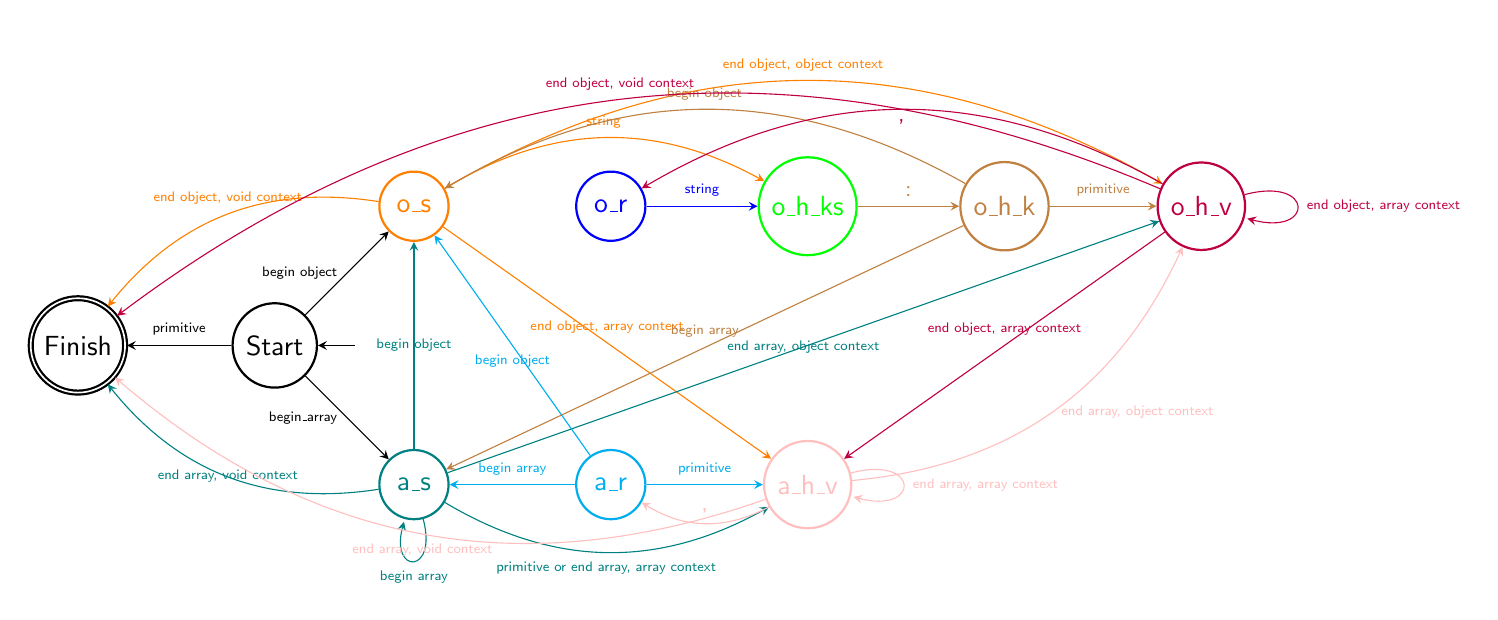
\begin{tikzpicture}[
        node distance=2.5cm, 
        on grid, 
        initial text=$ $, 
        ->,
        >=stealth,
        every state/.style={thick}]
        % States
        \node[state, initial, initial where=right] (entry) {Start};
        \node[state, left of=entry, accepting] (finish) {Finish};
        
        \node[state, above right of=entry, orange] (obj_start) {\objectstart};
        \node[state, right of=obj_start, blue] (obj_ready) {\objectready};
        \node[state, right of=obj_ready, green] (obj_has_key_string) {\objecthaskeystring};
        \node[state, right of=obj_has_key_string, brown] (obj_has_key) {\objecthaskey};
        \node[state, right of=obj_has_key, purple] (obj_has_value) {\objecthasvalue};
        
        \node[state, below right of=entry, teal] (array_start) {\arraystart};
        \node[state, right of=array_start, cyan] (array_ready) {\arrayready};
        \node[state, right of=array_ready, pink] (array_has_value) {\arrayhasvalue};
        % Edges
        \draw[->] (entry) edge node[left]{\tiny begin object} (obj_start);
        \draw[->] (entry) edge node[above]{\tiny primitive} (finish);
        
        \draw[->, orange] (obj_start) edge [bend left, above] node[above]{\tiny string} (obj_has_key_string);
        \draw[->, orange] (obj_start) edge [bend left, above] node[above]{\tiny end object, object context} (obj_has_value);
        \draw[->, orange] (obj_start) edge [above] node[above]{\tiny end object, array context} (array_has_value);
        \draw[->, orange] (obj_start) edge [bend right] node[above]{\tiny end object, void context} (finish);
        
        \draw[->, blue] (obj_ready) edge [above] node[above]{\tiny string} (obj_has_key_string);
        
        \draw[->, brown] (obj_has_key_string) edge node[above]{\footnotesize :} (obj_has_key);
        
        \draw[->, brown] (obj_has_key) edge node[above]{\tiny primitive} (obj_has_value);
        \draw[->, brown] (obj_has_key) edge[bend right] node[above]{\tiny begin object} (obj_start);
        \draw[->, brown] (obj_has_key) edge node[above]{\tiny begin array} (array_start);
        
        \draw[->, purple] (obj_has_value) edge[bend right] node[above]{\tiny end object, void context} (finish);
        \draw[->, purple] (obj_has_value) edge node[above]{\tiny end object, array context} (array_has_value);
        \draw[->, purple] (obj_has_value) edge[loop right] node[right]{\tiny end object, array context} (obj_has_value);
        \draw[->, purple] (obj_has_value) edge[bend right] node[below]{\footnotesize ,} (obj_ready);
        
        \draw[->, teal] (array_start) edge node{\tiny begin object} (obj_start);
        \draw[->, teal] (array_start) edge[bend right] node[below]{\tiny primitive or end array, array context} (array_has_value);
        \draw[->, teal] (array_start) edge node{\tiny end array, object context} (obj_has_value);
        \draw[->, teal] (array_start) edge[bend left] node{\tiny end array, void context} (finish);
        \draw[->, teal] (array_start) edge[loop below] node{\tiny begin array} (array_start);
        
        \draw[->, cyan] (array_ready) edge node[above]{\tiny begin array} (array_start);
        \draw[->, cyan] (array_ready) edge node[below]{\tiny begin object} (obj_start);
        \draw[->, cyan] (array_ready) edge node[above]{\tiny primitive} (array_has_value);
        
        \draw[->, pink] (array_has_value) edge[loop right] node[right]{\tiny end array, array context} (array_has_value);
        \draw[->, pink] (array_has_value) edge[bend right] node[right]{\tiny end array, object context} (obj_has_value);
        \draw[->, pink] (array_has_value) edge[bend left] node[below]{\tiny end array, void context} (finish);
        \draw[->, pink] (array_has_value) edge[bend left] node[above]{\footnotesize , } (array_ready);
        
        \draw[->] (entry) edge node[left]{\tiny begin\_array} (array_start);
      \end{tikzpicture}
    \end{figure}
  
  \section{States}
  
    \begin{description}
      \item[start] initial state of the composer;
      \item[error] the state the composer will be in if an error has occured; 
      \item[finish] the state the compoer will be in after the root object has
      been parsed;  
      \item[object start] the initial start of an object;
      \item[object has key string] the state in which the composer will be in 
      after receiving the string that represents the key;
      \item[object has key] the state in which the composer will be in after 
      receiving the key string and the key value separator 
      token;
      \item[object has value] the state in which the composer will be in after
      receiving a value;
      \item[object ready] the state in which the composer will be in after 
      receiving a value separator and is ready to start 
      taking a new key-value pair; 
      \item[array start] the inital state of an array;
      \item[array has value] the state in which the composer will be in after 
      receiving a value;  
      \item[array ready] the state in which the composer will be in after 
      receiving value separator and ready to take the next element; 
    \end{description}
    
    \begin{tabu} to \linewidth{ X[l] | X[l] }
      \thickhline
      \textbf{State} & \textbf{Shorthand} \\ \thickhline
      start & start \\ \hline
      error & error \\ \hline
      finish & finish \\ \hline
      object start & \objectstart \\ \hline
      object has key string & \objecthaskeystring \\ \hline
      object has key & \objecthaskey \\ \hline
      object has value & \objecthasvalue \\ \hline
      object ready & \objectready \\ \hline
      array start & \arraystart \\ \hline
      array has value & \arrayhasvalue \\ \hline
      array ready & a\_r \\ \thickhline
    \end{tabu}
  
  \section{Inputs}
  
    \begin{tabu} to \linewidth{ X[1,l] | X[3,l] }
      \thickhline
      \textbf{Input} & \textbf{Description} \\ \thickhline 
      begin\_object & true when the token is begin object \\ \hline
      begin\_array & true when the token is begin array \\ \hline
      end\_obj & true when the token is end object \\ \hline
      end\_array & true when the token is end array \\ \hline
      key\_value\_separator & true when the token is a key value separator \\ \hline
      value\_separator & true when the token is a value separator \\ \hline
      string & true when the token is string \\ \hline
      boolean & true when the token is boolean \\ \hline
      number & true when the token is number \\ \hline
      null & true when the token is null \\ \hline
      non\_string & true when the token is a primitive other than string \\ \hline
      primitive & true when the token is string, boolean, number, or null \\ \hline
      void\_context & true when there is no parent object \\ \hline
      obj\_context & true when the parent is an object \\ \hline
      array\_context & true when the parent is an array \\ \thickhline
    \end{tabu}
    
  \section{Transitions}
  
    \begin{itemize}
      \item \textbf{push stack}: add new item to the stack;
      \item \textbf{pop stack}: pop item from the stack and and insert the 
      item into the new top of the stack;
    \end{itemize}
    
    \begin{longtabu} to \linewidth{  X[1,l] | X[1,l] | X[3,l] | X[3,l] }
      \thickhline
      \textbf{From} & \textbf{To} & \textbf{Condition} & \textbf{Action} \\ \thickhline
      % start state's outbonding transitions
      \multicolumn{4}{c}{From \textbf{Start} State} \\ \thickhline
      start & finish & primitive & push stack \\ \hline 
      start & \objectstart & begin\_object & push stack \\ \hline
      start & \arraystart & begin\_array & push stack \\ \thickhline
      % object start state's outbonding transitions
      \multicolumn{4}{c}{From \textbf{Object Start} State} \\ \thickhline
      \objectstart & \objecthaskeystring & string & record key \\ \hline
      \objectstart & \objecthasvalue & end\_obj \& obj\_context & \\ \hline
      \objectstart & \arrayhasvalue & end\_obj \& array\_context & \\ \hline
      \objectstart & finish & end\_obj \& void\_context & \\ \hline
      \objectstart & error & else & \\ \thickhline
      % object ready state's outbonding transitions
      \multicolumn{4}{c}{From \textbf{Object Ready} State} \\ \thickhline
      \objectready & \objecthaskeystring & string & record key \\ \hline
      \objectready & error & else & \\ \thickhline
      % object has key string state's outbonding transitions
      \multicolumn{4}{c}{From \textbf{Object Has Key String} State} \\ \thickhline
      \objecthaskeystring & \objecthaskey & key\_value\_separator & record key \\ \hline
      \objecthaskeystring & error & else & \\ \thickhline
      % object has key state's outbonding transitions
      \multicolumn{4}{c}{From \textbf{Object Has Key} State} \\ \thickhline
      \objecthaskey & \objecthasvalue & primitive & push stack \\ \hline
      \objecthaskey & \objectstart & begin\_object & push stack \\ \hline
      \objecthaskey & \arraystart & begin\_arary & push stack \\ \hline
      \objecthaskey & error & else & \\ \thickhline
      % object has value state's outbonding transitions
      \multicolumn{4}{c}{From \textbf{Object Has Value} State} \\ \thickhline
      \objecthasvalue & \objectready & value\_separator & pop stack  \\ \hline
      \objecthasvalue & \objecthasvalue & end\_object \& object\_context & pop stack  \\ \hline
      \objecthasvalue & \arrayhasvalue & end\_object \& array\_context & pop stack \\ \hline
      \objecthasvalue & finish & end\_object \& void\_context & \\ \hline
      \objecthasvalue & erorr & else & \\ \thickhline
      % array start state's outbonding transitions
      \multicolumn{4}{c}{From \textbf{Array Start} State} \\ \thickhline
      \arraystart & \arraystart & begin\_array & push stack \\ \hline
      \arraystart & \objectstart & begin\_object & push stack \\ \hline
      \arraystart & \arrayhasvalue & primitive & push stack \\ \hline
      \arraystart & \objecthasvalue & end\_array \& object\_context & \\ \hline
      \arraystart & \arrayhasvalue & end\_array \& array\_context & \\ \hline
      \arraystart & finish & end\_array \& void\_context & \\ \hline
      \arraystart & eror & error & \\ \thickhline
      % array ready state's outbonding transitions
      \multicolumn{4}{c}{From \textbf{Array Ready} State} \\ \thickhline
      \arrayready & \objectstart & begin\_object & push stack \\ \hline
      \arrayready & \arraystart & begin\_array & push stack \\ \hline
      \arrayready & \arrayhasvalue & primitive & push stack \\ \hline
      \arrayready & error & else & \\ \thickhline
      % array has value state's outbonding transitions
      \multicolumn{4}{c}{From \textbf{Array Has Value} State} \\ \thickhline
      \arrayhasvalue & \arrayready & value\_separator & pop stack \\ \hline 
      \arrayhasvalue & \arrayhasvalue & end\_array \& array\_context & pop stack \\ \hline 
      \arrayhasvalue & \objecthasvalue & end\_array \& object\_context & pop stack \\ \hline 
      \arrayhasvalue & \objecthasvalue & end\_array \& void\_context & \\ \hline 
      \arrayhasvalue & error & else & \\ \thickhline 
    \end{longtabu}
\end{document}